\section{Charge Transfer Properties}
We have seen that the final structure of the pentacene systems becomes more ordered and crystal-like as the quenching time is increased. It would be good now to see how this affects the charge transfer properties. A key quantity governing charge transfer rates is the ratio between electronic coupling and reorganisation energy, $\frac{H_{ab}}{\lambda}$. Seeing as we have a single molecule system, by plotting the electronic coupling we can get a qualitative view of the charge transfer dynamics and see which paths are the most likely within the structure.
\subsection{Coupling Graphs}
In figure \ref{fig:crystalCouplingGraph} the graph of electronic couplings between molecules has been plotted for each of the quenched systems and a crystal system after a short equilibration run with MD. In this figure the centers of mass each molecule is represented by a small black dot and the calculated coupling value with a coloured line (red, green blue). That is, if 2 molecules have a non-negligible coupling between them they would be represented by 2 black dots with either a red, green or blue line connecting them. The couplings were calculated via the analytic overlap method \cite{gajdos_ultrafast_2014} and a pertinent cluster of molecules was selected for each quench time. For the 0ns and 1ns quench times this was simply a slice 1 molecule thick in the z dimension, containing a few hundred molecules. For the 10ns and 100ns quenched structures a reasonable cluster of molecules was chosen after applying a density based clustering algorithm on the superstructure. For the crystal a plane from the crystal was chosen. All panes in figure \ref{fig:crystalCouplingGraph} show the coupling of the selected system from an angle perpendicular to the plane of molecules.
\begin{figure}
	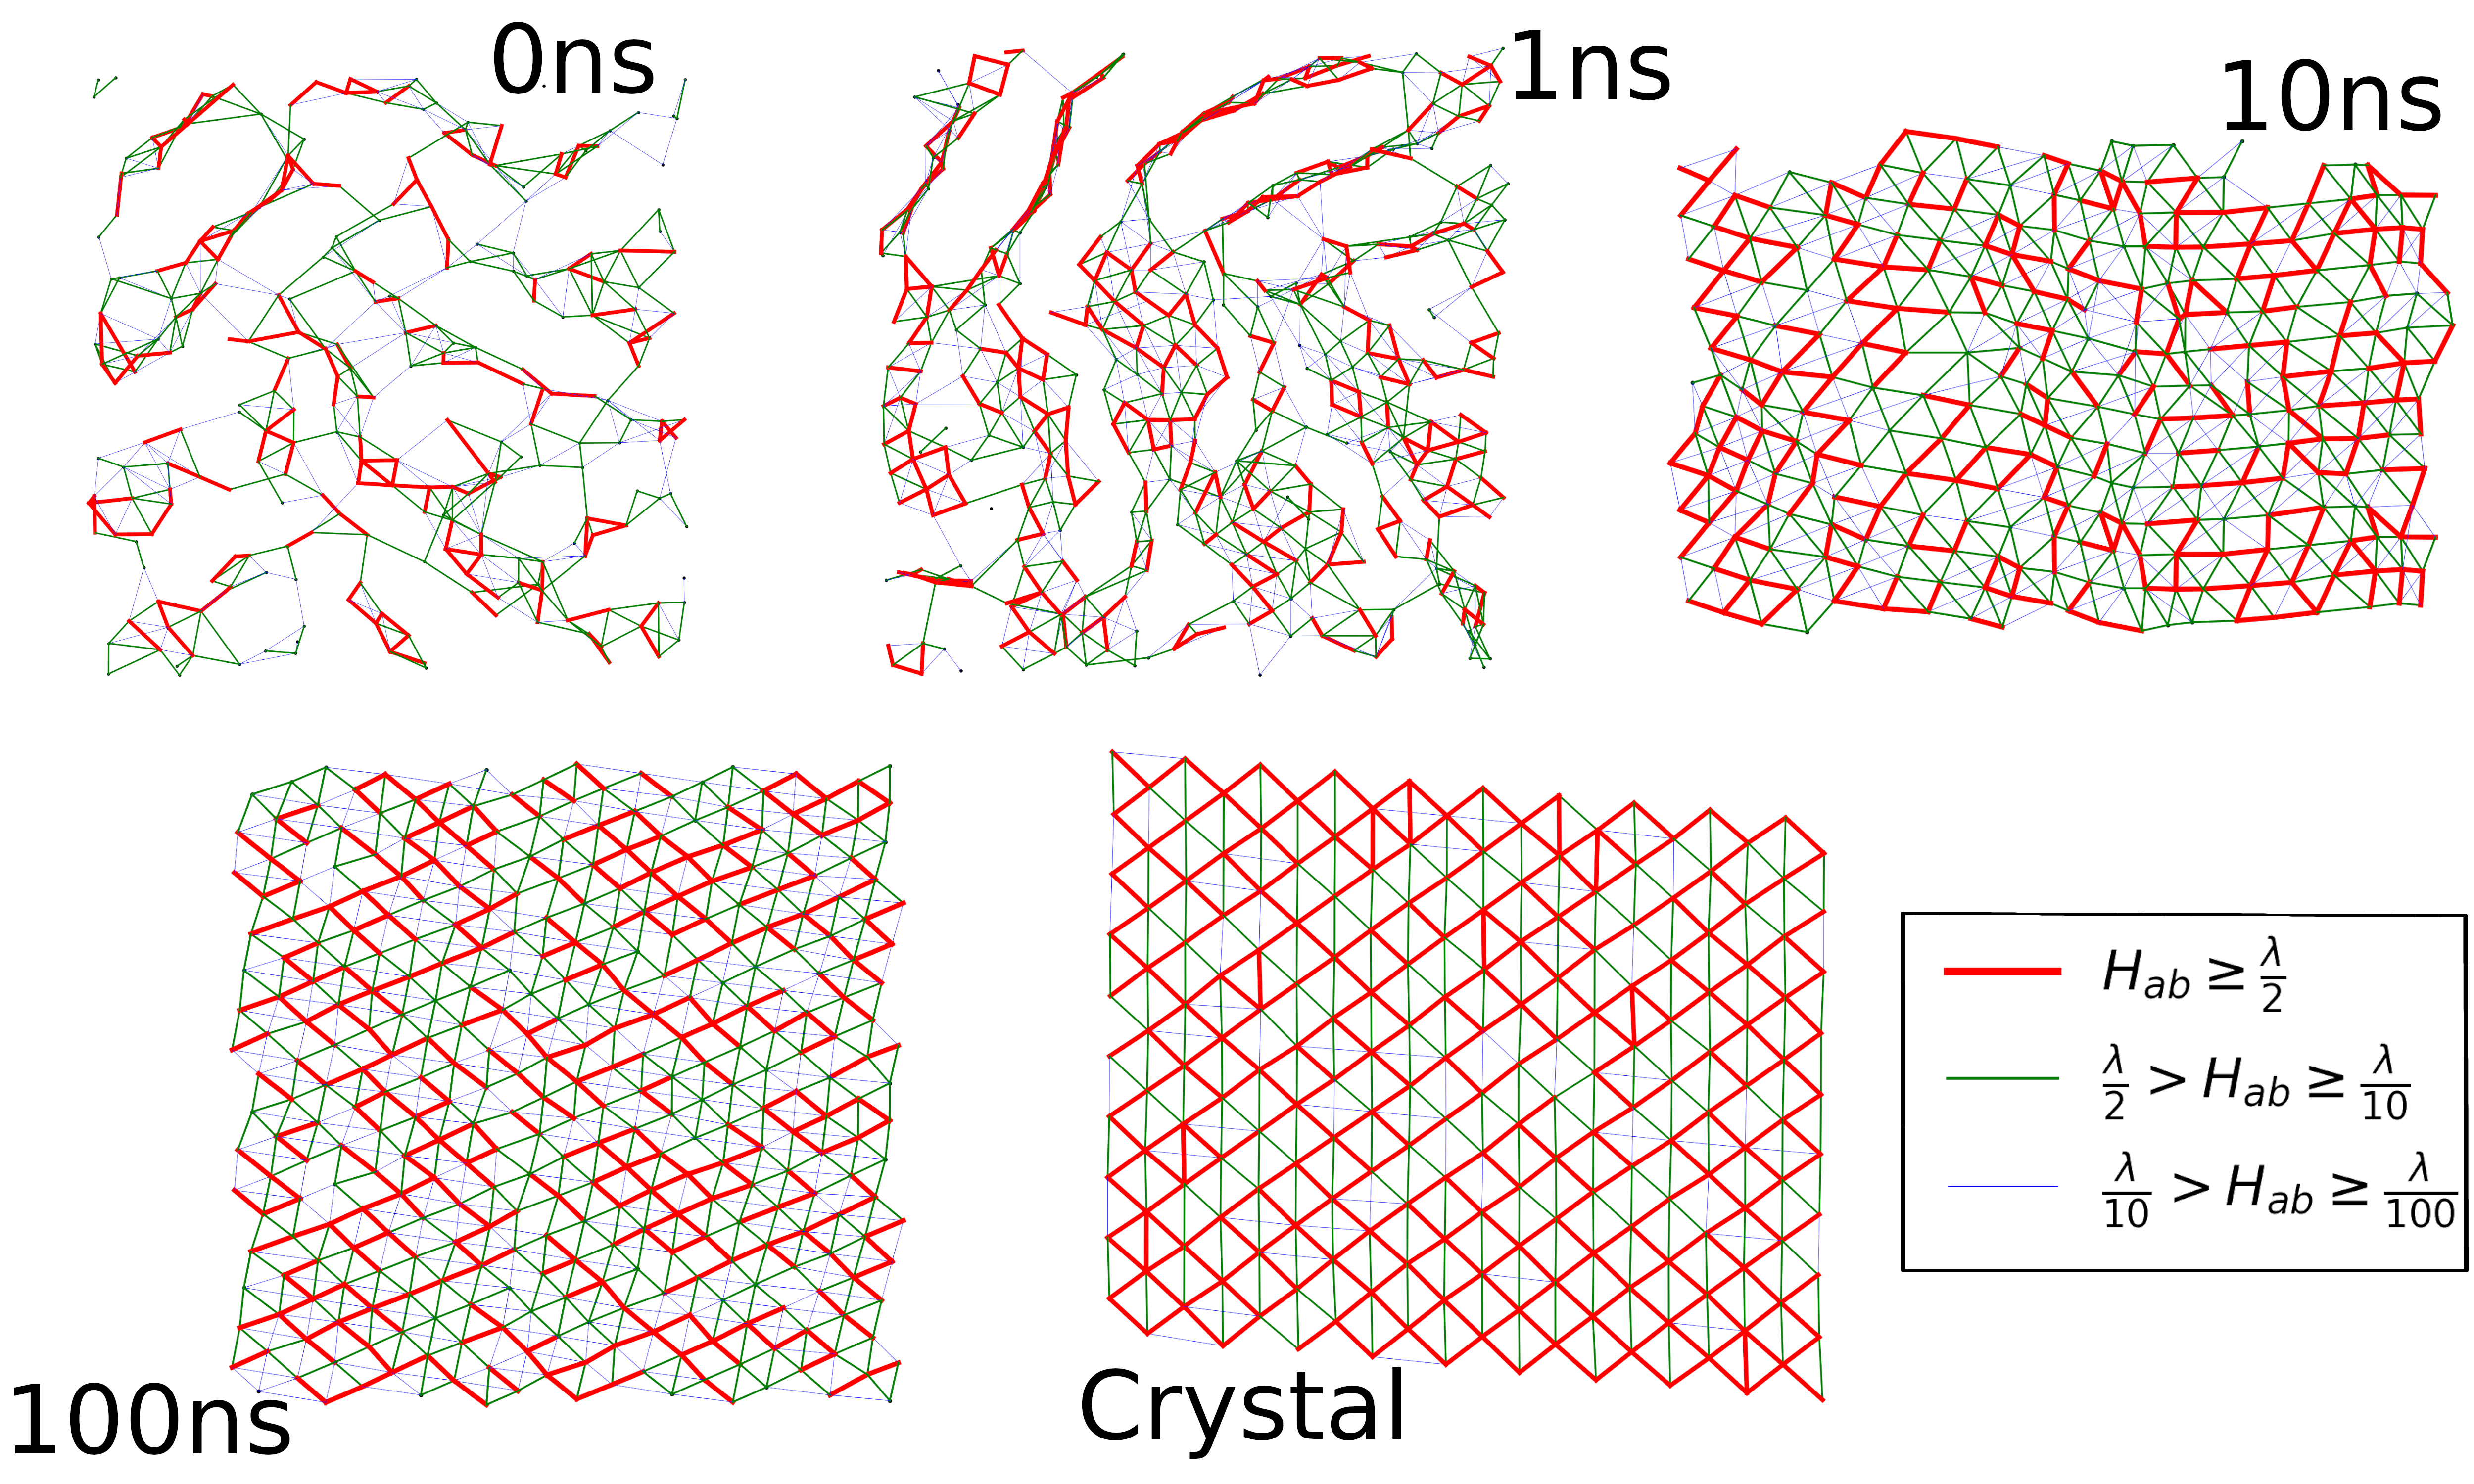
\includegraphics[width=\textwidth]{./img/CouplingPlots/CouplingGraphs_all.png}
	\caption{\label{fig:crystalCouplingGraph}A representative network of electronic coupling that each quenched structure has formed. Each structure is labelled by the quench time (e.g. 0ns, 1ns, 10ns, 100ns) or Crystal for a crystal after a short MD equilibration. Coupling strengths are categorised as high (red), medium (green) and low (blue). The definitions of the categories are given in the legend in the bottom right corner.}
\end{figure}
\\\\
We can see in the graph of the 0ns quenched structure there is very little order to the coupling network. Only very small fragments of high (red) coupling are formed and each one is connected via weak or medium coupling. We can define a 'high coupling fragment' as any set of molecules which can all be reached from any member of the set via an unbroken path of high coupling. The mean size of these high coupling fragments in the 0ns structure is 4.1 molecules and there are 503 of them. In this structure we would expect to see a localised polaron (over a $\sim$ 3 molecules) and low mobilities due to the lack of conductive channels in the structure. The mean size of fragments increases and the number of fragments decreases as we increase the quenching time as shown in table \ref{tab:cluster_sizes}.
\\
\begin{table}[h]
	\begin{tabular}{cccc}
		\textbf{Quench Time} [ns] & \textbf{Mean Fragment Size} & \textbf{Fragment Size Std Dev} & \textbf{Num Fragments} \\
		\hline &&&\\
		0 & 4.2 & 3.8 & 503 \\
		1 & 4.5 & 5.0 & 493 \\
		10 & 6.5 & 9.3 & 373 \\
		100 & 8.7 & 16.2 & 292 \\
		\hline &&&\\
	\end{tabular}
	\caption{\label{tab:cluster_sizes}The change in the number of high coupling fragments, and the mean and standard deviation of their size, found in each structure as the quenching time was varied.}
\end{table}
\\
We can see in table \ref{tab:cluster_sizes} that as the quenching time increases, the size of the highly coupled fragments (how many molecules are connected) increases and fewer of them are formed. The standard deviation also increases showing in the 0ns quenched structure most fragments are very small but as we increase the quench time we still get smaller fragments but much larger ones can now form too. These larger fragments can act as regions of high conductivity allowing much larger mobilities to be achieved than in the quicker quenching times.

\clearpage
\subsection{Molecular Dynamics without Partial Charges}


\label{sect:partial_charge_importance}

